%
% section 3.6.1
%
\subsection{Άμεση -- Έμμεση Δρομολόγηση}

Η βασική αρχή της δρομολόγησης είναι απλή: Ο αποστολέας δημιουργεί τα αυτοδύναμα πακέτα IP και εξετάζει την διεύθυνση προορισμού: αν είναι τοπική, βρίσκεται δηλ. στο ίδιο δίκτυο με αυτόν, δεν έχει να κάνει κάτι το ιδιαίτερο: αρκεί να δώσει το πακέτο στο παρακάτω επίπεδο που θα φροντίσει για την αποστολή στο φυσικό μέσο.  

Εάν η διεύθυνση προορισμού δεν είναι τοπική, ο αποστολέας αναζητά κατάλληλο δρομολογητή ο οποίος ελπίζει να βρίσκεται στη σωστή κατεύθυνση  προς τον προορισμό και στέλνει τα  πακέτα σε αυτόν.  Ο δρομολογητής εκτελεί ουσιαστικά την ίδια διαδικασία και το στέλνει σε ένα άλλο δρομολογητή κ.ο.κ. μέχρι το πακέτο να φτάσει σε ένα δρομολογητή που βρίσκεται στο ίδιο φυσικό δίκτυο με τον υπολογιστή προορισμού. Εκεί παραδίδεται το πακέτο.

\begin{figure}[!ht]
 \centering
 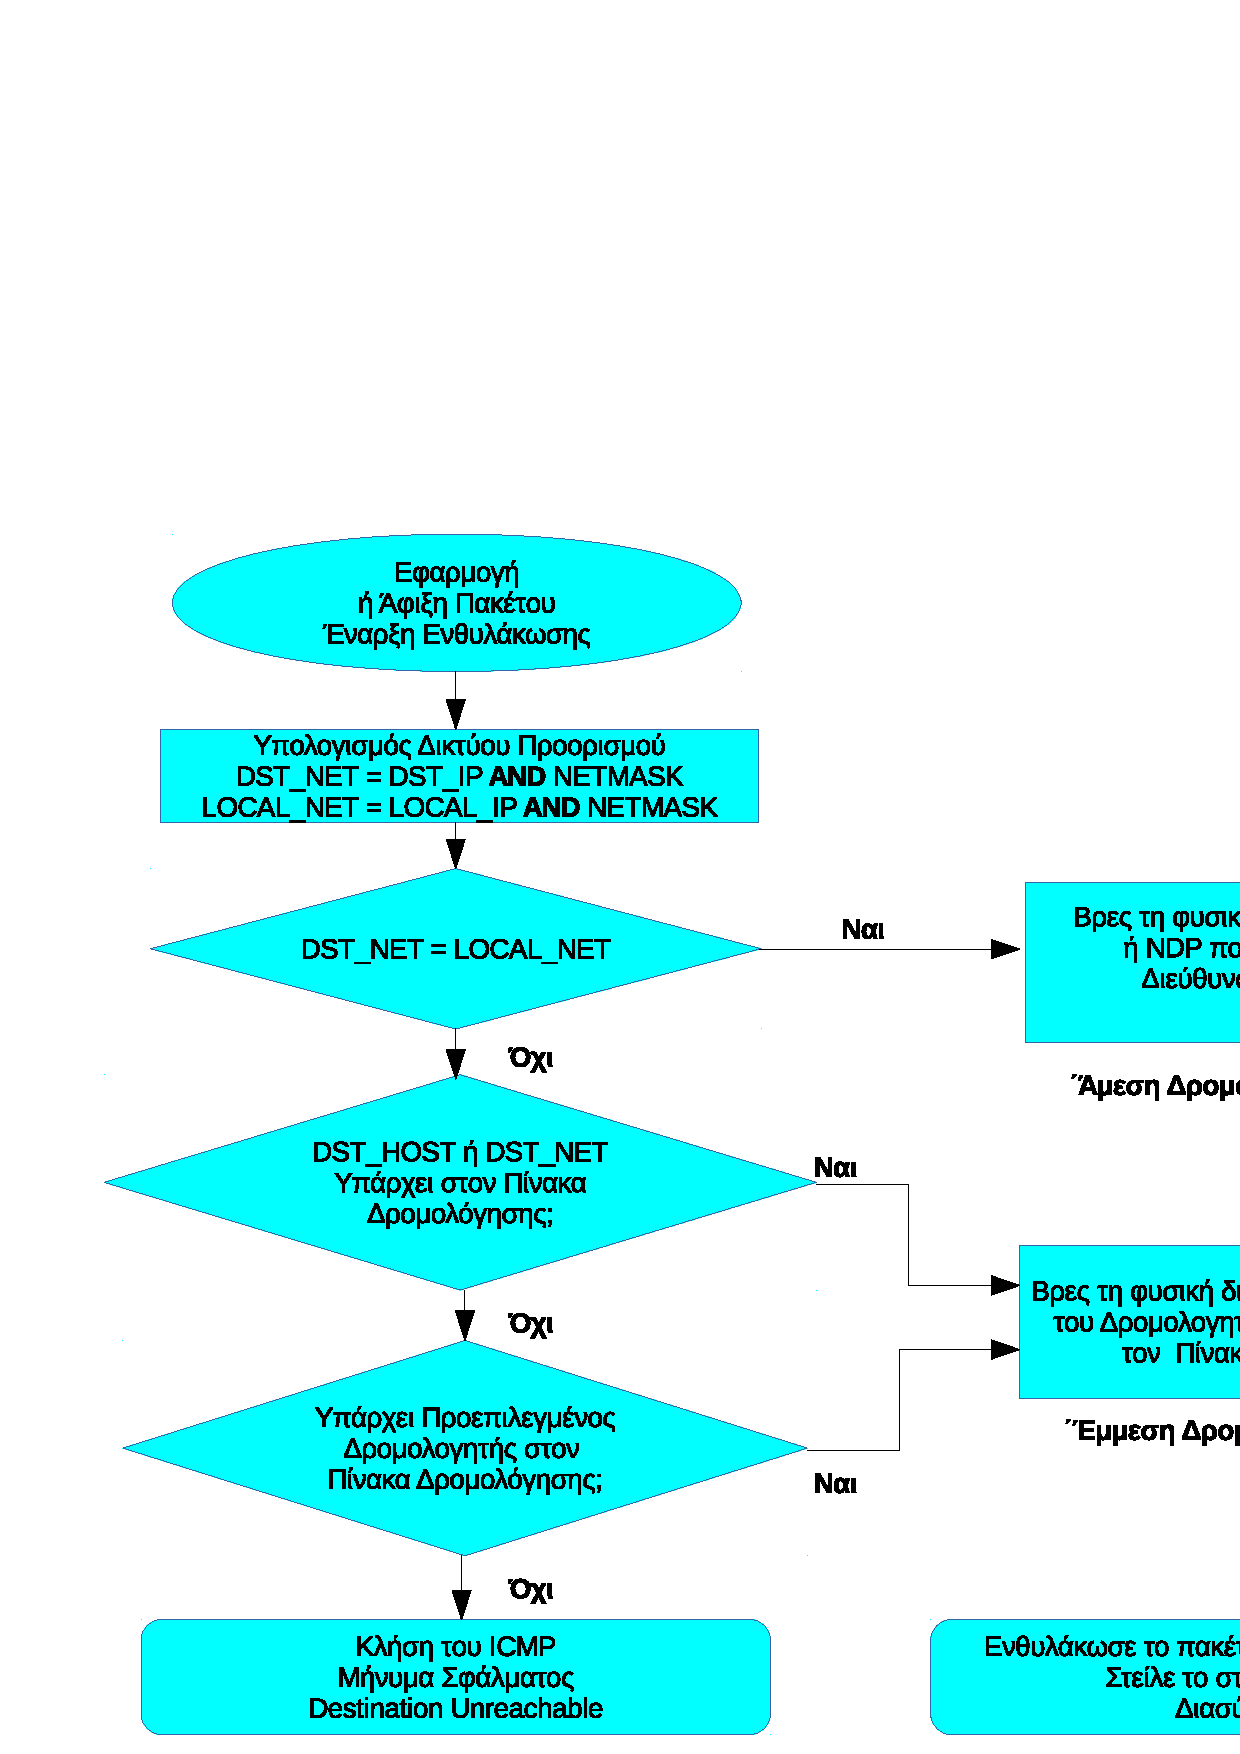
\includegraphics[width=0.95\textwidth]{images/chapter3/3-21}
 \caption {\textsl{Διαδικασία Δρομολόγησης Αυτοδύναμου Πακέτου}}
 \label{3-21}
\end{figure}


Με περισσότερες λεπτομέρειες, ακολουθείται η παρακάτω διαδικασία:

\begin{itemize}
\item Ο αποστολέας εκτελεί τη λογική πράξη \textbf{ΚΑΙ} μεταξύ της διεύθυνσης προορισμού και της μάσκας υποδικτύου. Προκύπτει έτσι η \emph{Διεύθυνση Δικτύου Προορισμού}.
\item Ο αποστολέας εξετάζει τη διεύθυνση δικτύου προορισμού: αν είναι στο  ίδιο φυσικό δίκτυο με αυτόν, δεν χρειάζεται να κάνει κάτι το ιδιαίτερο: η δρομολόγηση είναι \emph{άμεση}. Θα χρησιμοποιήσει το πρωτόκολλο ARP (ή NDP για IPv6) για να βρει τη φυσική διεύθυνση του υπολογιστή προορισμού και θα παραδώσει το πακέτο στο παρακάτω επίπεδο για να γίνει ενθυλάκωση του σε πλαίσιο και αποστολή στο φυσικό μέσο.
\item Αν η διεύθυνση δικτύου προορισμού δεν είναι ίδια με αυτή του αποστολέα, το πακέτο θα πρέπει να αποσταλεί σε ένα κατάλληλο δρομολογητή. Στην περίπτωση αυτή η δρομολόγηση είναι \emph{έμμεση}. Ο αποστολέας θα συμβουλευτεί τον πίνακα δρομολόγησης αναζητώντας μια εγγραφή που να ταιριάζει στον υπολογιστή προορισμού (DST\_HOST) ή στο δίκτυο προορισμού (DST\_NET). Αν βρει αυτή την εγγραφή, θα χρησιμοποιήσει το πρωτόκολλο ARP για να βρει τη φυσική διεύθυνση του αντίστοιχου δρομολογητή. Στη συνέχεια θα παραδώσει το πακέτο στο παρακάτω επίπεδο για να γίνει ενθυλάκωση του σε πλαίσιο και αποστολή στο φυσικό μέσο. Σημειώστε ότι στην έμμεση δρομολόγηση το πακέτο έχει τη λογική διεύθυνση του τελικού παραλήπτη αλλά το πλαίσιο τη φυσική διεύθυνση του δρομολογητή που θα αναλάβει την δρομολόγηση.
\item Αν ο πίνακας δρομολόγησης δεν περιέχει εγγραφή που να ταιριάζει με τη διεύθυνση του υπολογιστή προορισμού ή με τη διεύθυνση δικτύου του υπολογιστή προορισμού, ο αποστολέας θα αναζητήσει εγγραφή για \emph{προεπιλεγμένο δρομολογητή}. Σε ένα δίκτυο, ο προεπιλεγμένος δρομολογητής αναλαμβάνει τη δρομολόγηση όλων των πακέτων για τα οποία δεν υπάρχει πιο συγκεκριμένη καταχώριση στον πίνακα δρομολόγησης (το router με το οποίο συνδέεστε στο Internet είναι ο προεπιλεγμένος δρομολογητής για το οικιακό σας δίκτυο). Αν υπάρχει προεπιλεγμένος δρομολογητής, ο αποστολέας θα αναζητήσει τη φυσική του διεύθυνση μέσω του ARP και θα παραδώσει το πακέτο στο παρακάτω επίπεδο για να γίνει, όπως και προηγουμένως, ενθυλάκωση και αποστολή του στο φυσικό μέσο.
\item Αν δεν βρεθεί καμιά κατάλληλη καταχώριση στον πίνακα και ούτε υπάρχει προεπιλεγμένος δρομολογητής, το πακέτο δεν είναι δυνατόν να παραδοθεί: η δρομολόγηση είναι αδύνατη. Ο αποστολέας θα ειδοποιηθεί μέσω του πρωτοκόλλου ICMP ότι ο προορισμός δεν είναι προσβάσιμος. 
\end{itemize}

Η παραπάνω διαδικασία φαίνεται και ως διάγραμμα ροής στο σχήμα \ref{3-21}.